\chapter{Управляемая динамика квадрокоптера с поворотными роторами}

\section{Основные элементы конструкции квадрокоптера с поворотными роторами}

Основным элементом конструкции является корпус, из которого выходят лучи с закрепленными на концах двигателями с пропеллерами. Лучи расположены симметрично относительно корпуса аппарата и реализуют так называемую Х-схему. Смежные пропеллеры имеют противоположное направление вращения; первый и третий – пропеллеры левого вращения, а второй и четвертый – правого. Каждый из роторов может поворачиваться посредством сервопривода вокруг продольной оси луча. Общий вид аппарата представлен рисунке \ref{fig:tiltrotor_scheme}.

\section{Постановка задачи управления}

Считая заданной требуемую траекторию БЛА в координатном пространстве, положим целью управления обеспечение наперёд заданной траектории центра масс аппарата, а также требуемой ориентации. Такая постановка позволяет формализовать следующие задачи:
\begin{itemize}
\item приведение центра масс БЛА в н	екоторое наперёд заданное статичное положение;
\item стабилизация ориентации БЛА относительно некоторого наперёд заданного положения;
\item перемещение центра масс БЛА вдоль некоторой наперёд заданной (дискретным набором точек или как непрерывная функция координат от времени) траектории;
\item слежение за объектом, перемещающимся произвольным образом;
\item наведение камеры, установленной на БЛА на неподвижный или перемещающийся объект (то есть съёмка неподвижного объекта с разных ракурсов или слежение камерой за подвижным объектом).
\end{itemize}

Решение последней задачи в явном виде использует степени свободы, связанные с увеличением размерности вектора управляющих параметров. Стоит отметить, что квадрокоптер со стандартной конструкцией произвольный манёвр наведения камеры в точку с одновременным изменением высоты выполнить не способен.

\begin{figure}[h]
	\centering
	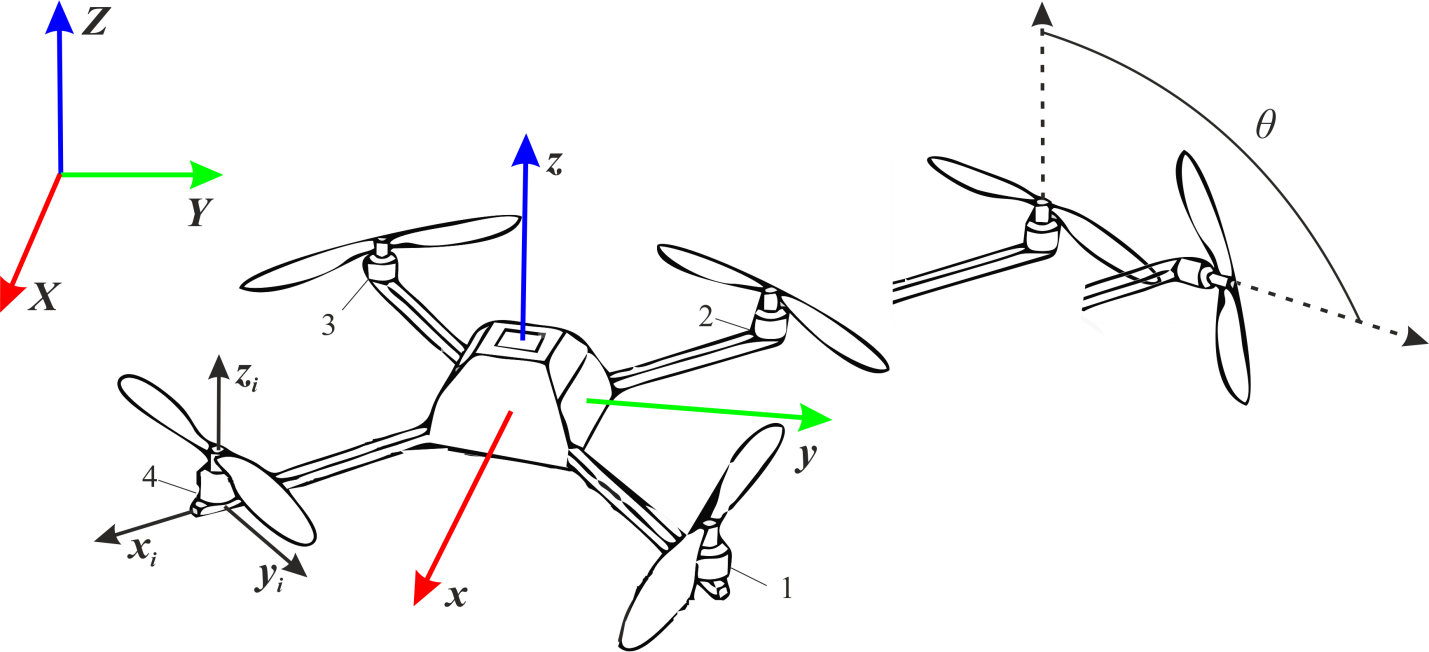
\includegraphics[scale=0.9]{tiltrotor_scheme}
	\caption{ -- Общая схема квадрокоптера с поворотными роторами}
	
	\label{fig:tiltrotor_scheme}
\end{figure}

\section{Математическая модель динамики аппарата}
Движение аппарата рассматривается относительно неподвижной инерциальной системы отсчета $I$, связанной с Землей (вращением Земли на характерных временах автономного полёта БЛА рассматриваемого класса принято пренебрегать).
Направление осей выбрано по схеме «Восток, Север, Верх» (ENU) -- ось \textbf{$X_I$} направлена на восток, ось \textbf{$Y_I$} -- на север, а ось \textbf{$Z_I$} -- от центра Земли.

Индексом $B$ обозначим жестко связанную с корпусом аппарата систему координат с началом в центре масс и осями, совпадающими с главными центральными осями инерции корпуса БЛА.
Для промежуточных выкладок нами будет использована ещё одна жестко связанная с корпусом система координат $B'$, полученная из $B$ поворотом вокруг оси $Z_B$ таким образом, что ось $X_B'$ направлена вдоль луча, несущего первый ротор согласно схеме \ref{fig:tiltrotor_scheme}.

Индексами $R_i$ будем обозначать системы координат, жестко связанные с роторами и совпадающие с их главными центральными осями инерции.

При записи векторов будем отмечать верхним индексом систему координат, в которой записано разложение вектора. Повороты систем координат друг относительно друга будем описывать кватернионами. Будем говорить, что кватернион $q_{IB}$ задаёт ориентацию системы координат $B$ относительно $I$ в том смысле, что разложения некоторого вектора $\bm{r}$ в этих двух базисах связаны соотношением
\begin{equation} \label{eq:m_quat}
\bm{r}^I = q_{IB} \circ \bm{r}^B \circ \tilde{q}_{IB}.
\end{equation}

При построении модели нами приняты следующие допущения: под ротором имеется в виду вращающаяся часть двигателя и пропеллер, которые считаются одним телом; корпус БЛА и каждый из четырех роторов считаются твердыми телами; крепление роторов к корпусу БЛА происходит в точках, совпадающих с центрами масс роторов. Помимо роторов в системе отсутствуют подвижные части; центры масс роторов лежат на окружности радиуса $L$, центр окружности совпадает с центром масс корпуса аппарата.

Положение БЛА в пространстве определяется радиус-вектором его центра масс $\bm{r}^I$ и кватернионом ориентации $q_{IB}$. Скорость центра масс аппарата равна
\begin{equation} \label{eq:m_vel}
\bm{v}^I = \dot{\bm{r}^I}.
\end{equation}
Изменение кватерниона ориентации аппарата определяется уравнением Пуассона
\begin{equation} \label{eq:m_puasson}
\dot{q}_{IB} = \frac{1}{2} {q}_{IB} \circ \bm{\Omega}^B,
\end{equation}
где $\bm{\Omega}_B$ – угловая скорость корпуса БЛА в проекции на собственные оси.

Движение центра масс БЛА определяется уравнением
\begin{equation} \label{eq:m_traslational_motion}
\ddot{\bm{r}} = M \bm{g}^I - \frac{1}{2} \rho C S_{\perp} |\bm{v}^I| \bm{v}^I + \sum_{i=1}^{4}{ { (-1)^{i+1} k \tilde \omega_i |\tilde \omega_i| \bm{e}^I_{z_i}}},
\end{equation}
где три члена в правой части соответствуют силе тяжести, силе аэродинамического сопротивления и создаваемой пропеллерами тяге, $M = m + \sum_{i=1}^{4}{m_i}$ – общая масса корпуса, $m_i$ – масса $i$-го ротора с пропеллером, $\bm g$ – ускорение свободного падения, $S_{\perp}$ – площадь миделева сечения корпуса аппарата, $C$ – аэродинамический коэффициент сопротивления воздуха, $\bm{e}^I_{z_i}$ – единичный вектор вдоль оси симметрии i-го ротора, $k$ – аэродинамический коэффициент, определяемый экспериментально; $\tilde \omega_i$ – скорость вращения i-го пропеллера.

Для описания вращательного движения воспользуемся динамическими уравнениям Эйлера
\begin{equation} \label{eq:m_rotational_motion}
\bm{\tau}^{B} =
\bm{J}_B\dot{\bm{\Omega}}^B + \bm{\Omega}^B \times \bm{J}_B{\bm{\Omega}^B},
\end{equation}
где $\bm{J}_B$ — тензор инерции корпуса в главных осях корпуса; $\bm{\tau}^{B}$ —
главный момент сил, действующий на корпус.

Главный момент сил складывается из моментов сил, действующих на корпус аппарата со стороны поворотных роторов с пропеллерами и внешних моментов:
\begin{equation} \label{eq:m_general_torq}
\bm{\tau}^{B} =
-\sum_{i=1}^{4} {\bm{\tau}^{B}_i} +
\sum_{i=1}^{4} {\bm{r}^B_i \times (-1)^{i+1} k \tilde \omega_i |\tilde \omega_i| \bm{e}^I_{z_i},}
\end{equation}
где $\bm{\tau}^{B}_i$ — моменты сил, действующие на роторы со стороны аппарата, $\bm{r}^B_i$ -- радиус вектор, проведенный из центра масс квадрокоптера $i$-тому к ротору. Вычислим угловую скорость $i$-го ротора в проекциях на оси $R_i$:
\begin{equation} \label{eq:m_prop_ang_vel}
\bm{\omega}^{R_i}_i =
q_{{R_i} B} \circ (\bm{\Omega}^B + \dot {\theta}_i \bm e^B_{r_i}) \circ \tilde {q}_{{R_i}B} +
\tilde \omega_i \bm{e}^{R_i}_{z_i},
\end{equation}
где $\bm e^B_{r_i}$ -- орт вектора $\bm{r}^B_i$, ${\theta}_i$ -- угол поворота $i$-того ротора. Запишем динамические уравнения Эйлера для ротров.
\begin{equation} \label{eq:m_rotors_dyn}
\bm{\tau}^{{R_i}}_i + \bm{\varsigma}^{{R_i}}_{i} = 
\bm{J}_{R_i}\dot{\bm{\omega}}^{R_i}_i + \bm{\omega}^{R_i}_i \times \bm{J}_{R_i}{\bm{\omega}^{R_i}_i},
\end{equation}
где $\bm{J}_{R_i}$ -- тензор инерции $i$-того ротора с пропеллером, записанный в собственных главных осях, $\bm{\varsigma}^{{R_i}}_{i}$ -- внешний момент силы, для которго запишем:
\begin{equation} \label{eq:m_ext_torq}
\begin{aligned}
&\bm{\varsigma}^{{R_i}}_{i} = -b \tilde \omega_i |\tilde \omega_i| \bm e^{R_i}_{r_i}\\
&\bm{\varsigma}^{B}_{i} = q_{ B {R_i}} \circ \bm{\varsigma}^{{R_i}}_{i} \circ \tilde q_{ B {R_i}}.
\end{aligned}
\end{equation}
Здесь $b$ -- аэродинамический коэффициент, определяемый экспериментально.

Окончательно уравнения вращательной динамики аппарата принимают вид:
\begin{equation} \label{eq:m_final_rotational_motion}
\begin{aligned}
\bm{J}_B\dot{\bm{\Omega}}^B + \bm{\Omega}^B \times \bm{J}_B{\bm{\Omega}^B} =
&\sum_{i=1}^{4} {\bm{r}^B_i \times
	(-1)^{i+1} k \tilde \omega_i |\tilde \omega_i| \bm{e}^I_{z_i}} + \\ +
\sum_{i=1}^{4} {\bm{\varsigma}^{{R_i}}_{i}} +
&\sum_{i=1}^{4} q_{ B {R_i}} \circ (\bm{J}_{R_i}\dot{\bm{\omega}}^{R_i}_i + \bm{\omega}^{R_i}_i \times \bm{J}_{R_i}{\bm{\omega}^{R_i}_i}) \circ \tilde q_{ B {R_i}}
\end{aligned}
\end{equation}
Уравнения (\ref{eq:m_vel}), (\ref{eq:m_puasson}), (\ref{eq:m_traslational_motion}) и (\ref{eq:m_final_rotational_motion}) составляют замкнутую систему, позволяющую моделировать динамику полета квадрокоптера с поворотными роторами.

\section{Синтез регулятора}

Пусть задана требуемая траектория центра масс аппарата $\bm r^0(t)$, а также требуемая ориентация $q^0(t)$. Обозначим  $\delta \bm r(t) = \bm r^0(t) - \bm r(t)$ и $\delta q(t) = q^0(t) \circ \tilde q(t)$, где $\delta \bm r$ и $\delta q$ определяют расхождение требуемой и текущей траектории БЛА в координатном пространстве, а $q = q_{IB}$.  В качестве переменных управления выберем скорости вращения пропеллеров ${\tilde \omega}_i$ и углы поворота роторов ${\theta}_i$:
\begin{equation} \label{eq:m_ctrl_out}
\begin{aligned}
	&\bm{u} = (\bm \omega_u, \bm \theta_u)^T,
	\\
	\bm \omega_u =
	(\tilde\omega_1 |\tilde\omega_1|,
	\tilde\omega_2 |\tilde\omega_2|&,
	\tilde\omega_3 |\tilde\omega_3|,
	\tilde\omega_4 |\tilde\omega_4|)^T,
	\quad
	\bm \theta_u = (\theta_1, \theta_2 , \theta_3 , \theta_4 )^T.
\end{aligned}
\end{equation}
Регуляторы, обеспечивающие необходимое управление по положению и ориентации могут быть построены, как
\begin{equation} \label{eq:m_reg}
\begin{aligned}
	\ddot{\bm{r}}(t)&=
	\ddot{\bm{r}}^0(t)+\bm{K}_{r1}(\dot{\bm{r}}(t)-\dot{\bm{r}}^0(t))+\bm{K}_{r2}\delta \bm r,\\
	\dot{\boldsymbol{\Omega}}(t)&=
	\dot{\boldsymbol{\Omega}}^0(t)+\bm{K}_{\Omega1}(\boldsymbol{\Omega}(t)-\boldsymbol{\Omega}^0(t))+\bm{K}_{\Omega2}\delta\bm{q},
\end{aligned}
\end{equation}
где $\delta \bm q$ -- векторная часть кватерниона $\delta q$,
$\ddot{\bm{r}}^0$, $\dot{\bm{r}}^0$, $\ddot{\bm{\Omega}}^0$, $\dot{\bm{\Omega}}^0$ -- целевое ускорение, скорость, угловое ускорение и угловая скорость соответственно,
$\bm K_{r1}$, $\bm K_{r2}$, $\bm K_{\Omega1}$, $\bm K_{\Omega2}$ -- диагональные матрицы коэффициентов, выбор которых согласно критерию Рауса-Гурвица гарантирует сходимость траектории аппарата к требуемой. Таким образом, для построения
контура управления, необходимо связать выход из регулятора с управляющими
параметрами, учесть присутствующие в системе ограничения на реализацию
управляющих воздействий, а также реализовать обратные связи.

\section{Обращение динамики модели}

Реализация контура управления с регуляторами (\ref{eq:m_reg}) требует обращения динамики системы, то есть определения значений всех управляющих параметров (\ref{eq:m_ctrl_out}) по выходу из регулятора (\ref{eq:m_reg}).
Для достижения этой цели преобразуем уравнения модели (\ref{eq:m_vel}), (\ref{eq:m_puasson}), (\ref{eq:m_traslational_motion}), (\ref{eq:m_final_rotational_motion}).
Запишем уравнения (\ref{eq:m_traslational_motion}) и (\ref{eq:m_final_rotational_motion}) в проекциях на оси системы координат $B'$.
Далее преобразуем уравнения таким образом, чтобы в правой части получившихся уравнений остались все члены, в которые явно входят управляющие параметры (\ref{eq:m_ctrl_out}), а все остальные члены перенесём в левую часть. Таким образом, получим систему уравнений
\begin{equation} \label{eq:m_dyn}
\begin{aligned}
&\bm F(\ddot{\bm r}, \dot{\bm r}, q) = k F_{thr} (\bm \theta_u) \bm \omega_u,\\
&\bm T(\dot{\bm \Omega}, \bm\Omega) = \Big(
kLT_{thr}(\bm\theta_u) - bT_{aero}(\bm\theta_u)
\Big)
\bm \omega_u.
\end{aligned}
\end{equation}
Матрицы в правой части уравнений принимают вид (\ref{eq:m_dyn}):
\begin{equation} \label{eq:m_dyn_matrixes}
\begin{aligned}
&F_{thr} =
\begin{bmatrix}
0&-s_2&0&s_4\\
-s_1&0&s_3&0\\
c_1&-c_2&c_3&-c_4
\end{bmatrix},
\\
\phantom{}
\\
&T_{thr} =
\begin{bmatrix}
0&-c_2&0&c_4\\
-c_1&0&c_3&0\\
-s_1&s_2&-s_3&s_4
\end{bmatrix},
\\
\phantom{}
\\
&T_{aero} =
\begin{bmatrix}
0&s_2&0&-s_4\\
-s_1&0&s_3&0\\
c_1&c_2&c_3&c_4
\end{bmatrix},
\end{aligned}
\end{equation}
где $c_i = cos(\theta_i)$, $s_i = sin(\theta_i)$.

Система (\ref{eq:m_dyn}) недоопределена и неленийна относительно компонент $\bm \theta_u$, что значительно затрудняет ее аналитическое решение. Доопределим систему, используя выражения для распределения вертикальных составляющих сил и моментов между парами двигателей, расположенных на параллельных лучах
\begin{equation} \label{eq:m_dyn_balance_1}
\begin{aligned}
&k \tilde\omega_1 |\tilde\omega_1| c_1 + k \tilde\omega_3 |\tilde\omega_3| c_3 =
\frac{1}{2} \bm F_z + \epsilon_F,
\\
&\tilde\omega_1 |\tilde\omega_1| (bc_1 - kLs_1)
+ \tilde\omega_3 |\tilde\omega_3| (bc_3 - kLs_3) =
\frac{1}{2} \bm T_z + \epsilon_T,
\end{aligned}
\end{equation}


\begin{equation} \label{eq:m_dyn_balance_2}
\begin{aligned}
&k \tilde\omega_2 |\tilde\omega_2| c_2 + k \tilde\omega_4 |\tilde\omega_4| c_4 =
-\frac{1}{2} \bm F_z + \epsilon_F,
\\
&\tilde\omega_2 |\tilde\omega_2| (bc_2 + kLs_2)
+ \tilde\omega_4 |\tilde\omega_4| (bc_4 + kLs_4) =
\frac{1}{2} \bm T_z - \epsilon_T,
\end{aligned}
\end{equation}
где $\epsilon_F$ и $\epsilon_F$ -- балансировочные параметры.

Полученная система уравнений (\ref{eq:m_dyn}), (\ref{eq:m_dyn_balance_1}) имеет аналитическое решение:
\begin{equation} \label{eq:m_dyn_resolve}
\nonumber
\begin{aligned}
&\tilde\omega_i |\tilde\omega_i| =
\frac{(-1)^{i+1}}{2kL}\Big(
A^2_i(\bm F, \bm T, \epsilon_F, \epsilon_T) + 
B^2_i(\bm F, \bm T, \epsilon_F, \epsilon_T)
\Big)^{\frac{1}{2}},
\\
\phantom{}
\\
&\theta_i = 
2 arctg\Bigg[ (-1)^{i+1}
\frac{A_i(\bm F, \bm T, \epsilon_F, \epsilon_T) -
\Big(A^2_i(\bm F, \bm T, \epsilon_F, \epsilon_T) +
B^2_i(\bm F, \bm T, \epsilon_F, \epsilon_T)
\Big)^{\frac{1}{2}}}
{B_i(\bm F, \bm T, \epsilon_F, \epsilon_T)}
\Bigg],
\end{aligned}
\end{equation}
где $A_i(\bm F, \bm T, \epsilon_F, \epsilon_T)$ и
$B_i(\bm F, \bm T, \epsilon_F, \epsilon_T)$
-- скалярные функции, куда линейно входят компоненты $\bm F$ и $\bm T$. Таким образом, полученные выражения связывают выход регулятора с управляющими параметрами при наличии обратной связи. 

\section{Введение ограничений на компоненты вектора упраляющих параметров}

Рассмотрим возможные ограничения на вектор управляющих параметров, а именно на максимальную скорость вращения роторов с пропеллерами и на углы отклонения сервоприводов. Пусть 

\begin{equation} \label{eq:m_dyn_resolve}
\nonumber
\begin{aligned}
&0< (-1)^{i+1} \tilde \omega_i |\tilde\omega_i| < \tilde \omega_{max}^2,
\\
&|\theta_i| < \theta_{max} < \pi.
\end{aligned}
\end{equation}
Используя аналитические выражения для компонент вектора управляющего воздействия [Поле], можно переписать ограничения [Поле] в виде 
